%%%%%%%%%%%%%%%%%%%%%%%%%%%%%%%%%%%%%%%%%
% Programming/Coding Assignment
% LaTeX Template
%
% This template has been downloaded from:
% http://www.latextemplates.com
%
% Original author:
% Ted Pavlic (http://www.tedpavlic.com)
%
% Note:
% The \lipsum[#] commands throughout this template generate dummy text
% to fill the template out. These commands should all be removed when 
% writing assignment content.
%
% This template uses a Perl script as an example snippet of code, most other
% languages are also usable. Configure them in the "CODE INCLUSION 
% CONFIGURATION" section.
%
%%%%%%%%%%%%%%%%%%%%%%%%%%%%%%%%%%%%%%%%%

%----------------------------------------------------------------------------------------
%	PACKAGES AND OTHER DOCUMENT CONFIGURATIONS
%----------------------------------------------------------------------------------------

\documentclass{article}

\usepackage{fancyhdr} % Required for custom headers
\usepackage{lastpage} % Required to determine the last page for the footer
\usepackage{extramarks} % Required for headers and footers
\usepackage[usenames,dvipsnames]{color} % Required for custom colors
\usepackage{graphicx} % Required to insert images
\usepackage{subcaption}
\usepackage{listings} % Required for insertion of code
\usepackage{courier} % Required for the courier font
\usepackage{lipsum} % Used for inserting dummy 'Lorem ipsum' text into the template
\usepackage{amsfonts}
\usepackage{amssymb}
\usepackage{amsmath}
\usepackage{enumerate}
\usepackage{soul}
%Code for including Python code in Latex - outlined on the Piazza forum post, taken from Stackoverflow

\usepackage{enumitem}
\usepackage[utf8]{inputenc}
\definecolor{dkgreen}{rgb}{0,0.6,0}
\definecolor{gray}{rgb}{0.5,0.5,0.5}
\definecolor{mauve}{rgb}{0.58,0,0.82}

\lstset{frame=tb,
  language=Python,
  aboveskip=3mm,
  belowskip=3mm,
  showstringspaces=false,
  columns=flexible,
  basicstyle={\small\ttfamily},
  numbers=none,
  numberstyle=\tiny\color{gray},
  keywordstyle=\color{blue},
  commentstyle=\color{dkgreen},
  stringstyle=true{mauve},
  breaklines=true,
  breakatwhitespace=true,
  tabsize=3
}

% Margins
\topmargin=-0.45in
\evensidemargin=0in
\oddsidemargin=0in
\textwidth=6.5in
\textheight=9.0in
\headsep=0.25in

% Paragraph spacing
\setlength{\parskip}{10pt}


\linespread{1.1} % Line spacing

% Set up the header and footer
\pagestyle{fancy}
\lhead{\hmwkAuthorName} % Top left header
\chead{\hmwkClass\ (\hmwkClassTime): \hmwkTitle} % Top center head
%\rhead{\firstxmark} % Top right header
\lfoot{\lastxmark} % Bottom left footer
\cfoot{} % Bottom center footer
\rfoot{Page\ \thepage\ of\ \protect\pageref{LastPage}} % Bottom right footer

\setlength\parindent{0pt} % Removes all indentation from paragraphs

%----------------------------------------------------------------------------------------
%	CODE INCLUSION CONFIGURATION
%----------------------------------------------------------------------------------------

\definecolor{MyDarkGreen}{rgb}{0.0,0.4,0.0} % This is the color used for comments
\lstloadlanguages{Perl} % Load Perl syntax for listings, for a list of other languages supported see: ftp://ftp.tex.ac.uk/tex-archive/macros/latex/contrib/listings/listings.pdf
\lstset{language=Perl, % Use Perl in this example
        frame=single, % Single frame around code
        basicstyle=\small\ttfamily, % Use small true type font
        keywordstyle=[1]\color{Blue}\bf, % Perl functions bold and blue
        keywordstyle=[2]\color{Purple}, % Perl function arguments purple
        keywordstyle=[3]\color{Blue}\underbar, % Custom functions underlined and blue
        identifierstyle=, % Nothing special about identifiers                                         
        commentstyle=\usefont{T1}{pcr}{m}{sl}\color{MyDarkGreen}\small, % Comments small dark green courier font
        stringstyle=\color{Purple}, % Strings are purple
        showstringspaces=false, % Don't put marks in string spaces
        tabsize=5, % 5 spaces per tab
        %
        % Put standard Perl functions not included in the default language here
        morekeywords={rand},
        %
        % Put Perl function parameters here
        morekeywords=[2]{on, off, interp},
        %
        % Put user defined functions here
        morekeywords=[3]{test},
       	%
        morecomment=[l][\color{Blue}]{...}, % Line continuation (...) like blue comment
        numbers=left, % Line numbers on left
        firstnumber=1, % Line numbers start with line 1
        numberstyle=\tiny\color{Blue}, % Line numbers are blue and small
        stepnumber=5 % Line numbers go in steps of 5
}

% Creates a new command to include a perl script, the first parameter is the filename of the script (without .pl), the second parameter is the caption
\newcommand{\perlscript}[2]{
\begin{itemize}
\item[]\lstinputlisting[caption=#2,label=#1]{#1.pl}
\end{itemize}
}

%----------------------------------------------------------------------------------------
%	DOCUMENT STRUCTURE COMMANDS
%	Skip this unless you know what you're doing
%----------------------------------------------------------------------------------------

% Header and footer for when a page split occurs within a problem environment
\newcommand{\enterProblemHeader}[1]{
%\nobreak\extramarks{#1}{#1 continued on next page\ldots}\nobreak
%\nobreak\extramarks{#1 (continued)}{#1 continued on next page\ldots}\nobreak
}

% Header and footer for when a page split occurs between problem environments
\newcommand{\exitProblemHeader}[1]{
%\nobreak\extramarks{#1 (continued)}{#1 continued on next page\ldots}\nobreak
%\nobreak\extramarks{#1}{}\nobreak
}

\setcounter{secnumdepth}{0} % Removes default section numbers
\newcounter{homeworkProblemCounter} % Creates a counter to keep track of the number of problems
\setcounter{homeworkProblemCounter}{-1}

\newcommand{\homeworkProblemName}{}
\newenvironment{homeworkProblem}[1][Problem \arabic{homeworkProblemCounter}]{ % Makes a new environment called homeworkProblem which takes 1 argument (custom name) but the default is "Problem #"
\stepcounter{homeworkProblemCounter} % Increase counter for number of problems
\renewcommand{\homeworkProblemName}{#1} % Assign \homeworkProblemName the name of the problem
\section{\homeworkProblemName} % Make a section in the document with the custom problem count
\enterProblemHeader{\homeworkProblemName} % Header and footer within the environment
}{
\exitProblemHeader{\homeworkProblemName} % Header and footer after the environment
}

\newcommand{\problemAnswer}[1]{ % Defines the problem answer command with the content as the only argument
\noindent\framebox[\columnwidth][c]{\begin{minipage}{0.98\columnwidth}#1\end{minipage}} % Makes the box around the problem answer and puts the content inside
}

\newcommand{\homeworkSectionName}{}
\newenvironment{homeworkSection}[1]{ % New environment for sections within homework problems, takes 1 argument - the name of the section
\renewcommand{\homeworkSectionName}{#1} % Assign \homeworkSectionName to the name of the section from the environment argument
\subsection{\homeworkSectionName} % Make a subsection with the custom name of the subsection
\enterProblemHeader{\homeworkProblemName\ [\homeworkSectionName]} % Header and footer within the environment
}{
\enterProblemHeader{\homeworkProblemName} % Header and footer after the environment
}

%----------------------------------------------------------------------------------------
%	NAME AND CLASS SECTION
%----------------------------------------------------------------------------------------

\newcommand{\hmwkTitle}{Bonus 1} % Assignment title
\newcommand{\hmwkDueDate}{Monday,\ February\ 5,\ 2018} % Due date
\newcommand{\hmwkClass}{CSC2515} % Course/class
\newcommand{\hmwkClassTime}{L0101} % Class/lecture time
\newcommand{\hmwkAuthorName}{Matthew Wong, 998803932} % Your name

%----------------------------------------------------------------------------------------
%	TITLE PAGE
%----------------------------------------------------------------------------------------

\title{
\vspace{2in}
\textmd{\textbf{\hmwkClass:\ \hmwkTitle}}\\
\normalsize\vspace{0.1in}\small{Due\ on\ \hmwkDueDate}\\
\vspace{0.1in}
\vspace{3in}
}

\author{\textbf{\hmwkAuthorName}}
%\date{} % Insert date here if you want it to appear below your name

%----------------------------------------------------------------------------------------

\begin{document}

\maketitle
\clearpage
%----------------------------------------------------------------------------------------
%	Introduction
%----------------------------------------------------------------------------------------

\begin{homeworkProblem}

\noindent \textit{Introduction and Readme}

Attached, you will find the \textit{knn.py} and associated Latex files for the write-up.  Code was written in Python 3.5 with the relevant numpy, ski-kit learn and matplotlib libraries.  You can execute the code by simply running python knn.py in a command line - the images will be saved to the current local directory.

\end{homeworkProblem}
\clearpage
%----------------------------------------------------------------------------------------
%	PROBLEM 1
%----------------------------------------------------------------------------------------

% To have just one problem per page, simply put a \clearpage after each problem

\begin{homeworkProblem}

\noindent \textit{kNN Investigation}

The purpose of this report is to outline instances where the performance of the kNN algorithm \textit{increases} with increasing $k$.  To highlight such an instance, three datasets were created using a normal random distribution.  Out of the 3 instances, 2 were centered at the same mean, $\mu$ while the third was centered much farther away.  Of the two centered at the same $\mu$, the difference in standard deviations were large.  Figure 1 is an illustration of the distribution of data.

\begin{figure}[!ht]\centering
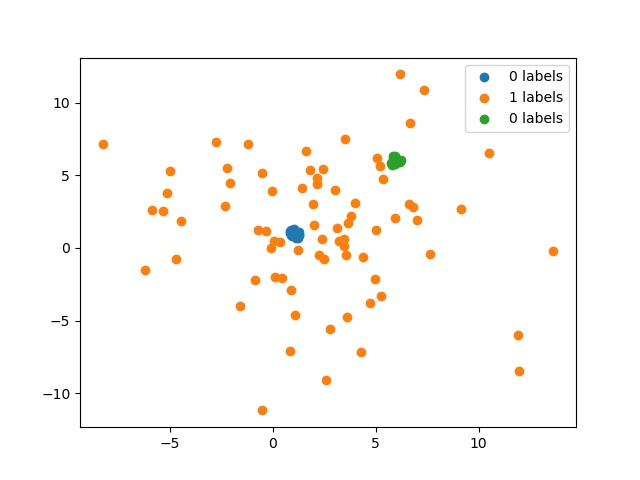
\includegraphics[scale=0.5]{Data_plot.jpg}
\caption{Randomly generated datasets, based on normal distributions}
\end{figure}
For the 0 labels, a small number of 0's is located near the 1 labels - the intuition here is that at low $k$ values, performance would drop.  At higher $k$ values, with a majority voting scheme, the "far-away" 0 labels would have more weight in the decision process and since they are so close to each other (e.g. small $\mu$) they would be considered over the 1-labelled points.  This is indeed the case as shown in Figure 2 as there were two increases - one at $k \approx 50$ and the other at $k \approx 70$.  Code for this experiment is located on the following page.

\begin{center}
\begin{figure}[!ht]\centering
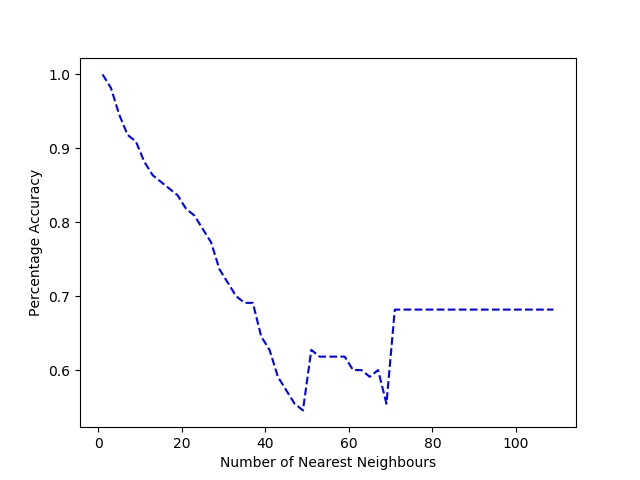
\includegraphics[scale=0.5]{Performance_Chart.jpg}
\caption{Percentage Accuracy of dataset vs. \# of nearest neighbours}
\end{figure}
\end{center}

\begin{lstlisting}
from sklearn.neighbors import KNeighborsClassifier
from sklearn.metrics import accuracy_score
import numpy as np
import matplotlib.pyplot as plt
#Set up seed and datasets
np.random.seed(1)
x1 = np.random.normal(loc = 1.0, scale = 0.15,size=(25,2))
x2 = np.random.normal(loc = 1.0, scale = 5.0,size=(75,2))
x3 = np.random.normal(loc = 6.0, scale = 0.15,size = (10,2))
#Plot and save the data
plt.scatter(x1[:,0],x1[:,1],label= "0 labels")
plt.scatter(x2[:,0],x2[:,1],label = "1 labels")
plt.scatter(x3[:,0],x3[:,1],label = "0 labels")
plt.legend()
plt.savefig('Data_plot.jpg')
plt.close()
#Stacking the matrices for X
x = np.vstack((x1,x2))
x = np.vstack((x,x3))
#Generate corresponding labels for clusters
y1 = np.zeros((25))
y2 = np.ones((75))
y3 = np.zeros((10))
#Stacking the labels
y = np.hstack((y1,y2))
y = np.hstack((y,y3))
#Stacking the matrices together
y = y[:,np.newaxis]
complete = np.hstack((x,y))
#Shuffle the matrix
np.random.shuffle(complete)
#Get the labels
labels = complete[:,-1]
#Get the data
complete = complete[:,:-1]
#KNN implementation
k_values, accuracy = [],[]
i = 1
while i < complete.shape[0]:
    knn = KNeighborsClassifier(n_neighbors=i)
    knn.fit(complete, labels)
    y_pred = knn.predict(complete)
    k_values.append(i)
    accuracy.append((accuracy_score(labels,y_pred)))
    i+=2
#Plotting the data
x_axis = k_values
y_axis = accuracy
plt.xlabel("Number of Nearest Neighbours")
plt.ylabel("Percentage Accuracy")
plt.plot(x_axis, y_axis, 'b--')
plt.savefig('Performance_Chart.jpg')

\end{lstlisting}
To test if this was just a product of noise, random seeds were selected:

\begin{center}
\begin{figure}[!ht]\centering
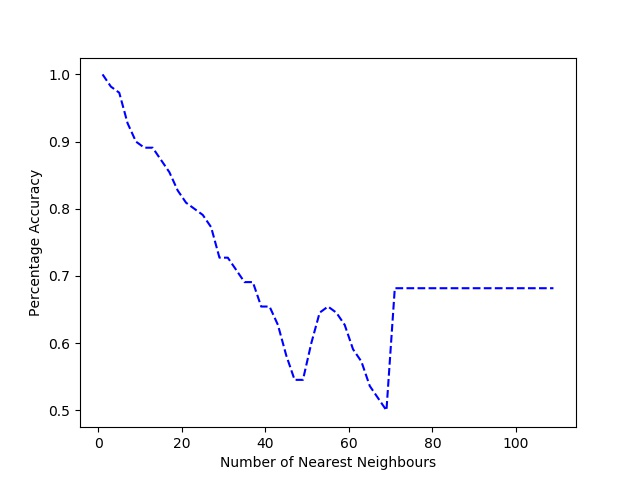
\includegraphics[scale=0.5]{Performance_Chart0.jpg}
\caption{Percentage Accuracy of dataset vs. \# of nearest neighbours, seed = 5}
\end{figure}
\end{center}

\begin{center}
\begin{figure}[!ht]\centering
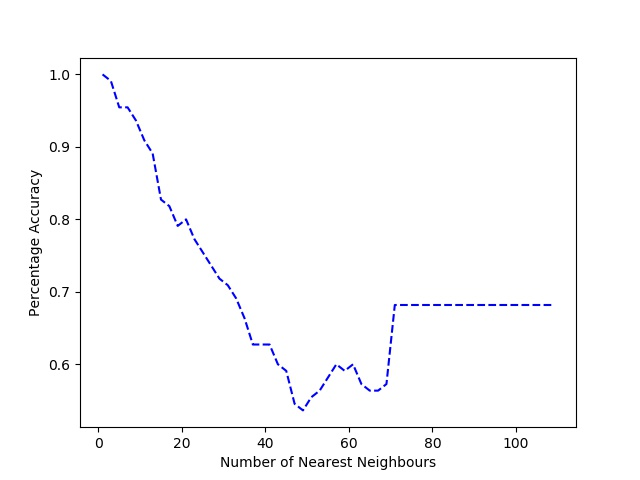
\includegraphics[scale=0.5]{Performance_Chart1.jpg}
\caption{Percentage Accuracy of dataset vs. \# of nearest neighbours, seed = 10}
\end{figure}
\end{center}

\begin{center}
\begin{figure}[!ht]\centering
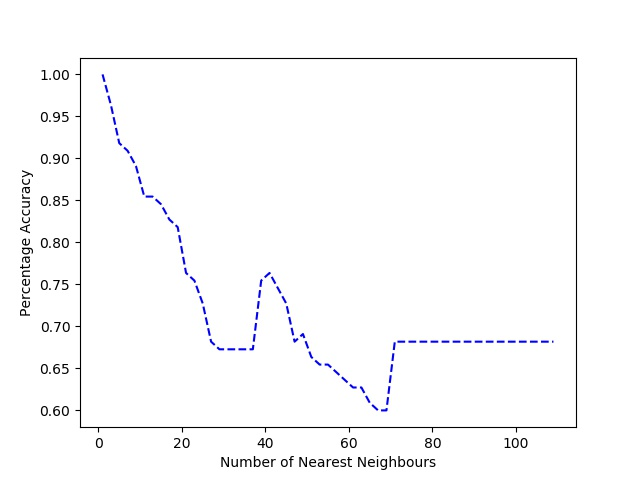
\includegraphics[scale=0.5]{Performance_Chart2.jpg}
\caption{Percentage Accuracy of dataset vs. \# of nearest neighbours, seed = 50}
\end{figure}
\end{center}

\begin{center}
\begin{figure}[!ht]\centering
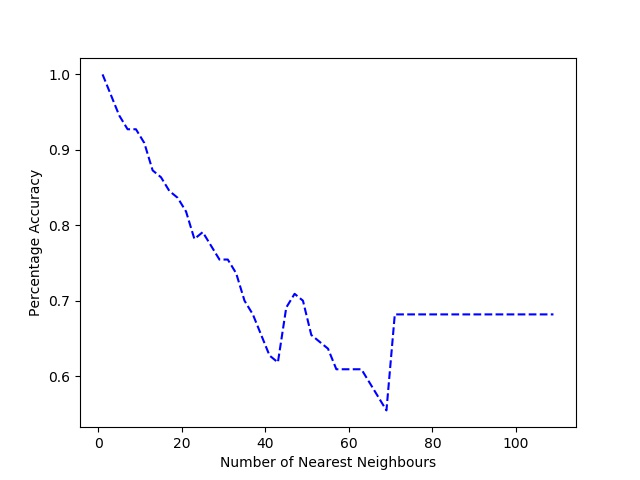
\includegraphics[scale=0.5]{Performance_Chart3.jpg}
\caption{Percentage Accuracy of dataset vs. \# of nearest neighbours, seed = 100}
\end{figure}
\end{center}

\end{homeworkProblem}

\end{document}